\chapter{Specyfikacja wewnętrzna}
\label{ch:05}

\section{Architektura systemu}

% \note{W tej części pracy należy opisać, jakie komponenty składają się na system. Należy zaznaczyć, jakie są relacje między nimi. Można również opisać, jakie wzorce projektowe zostały zastosowane. Głównie chodzi o to, aby czytelnik mógł zrozumieć, jak działa system.}

Kompletny system składa się z czterech głównych komponentów, które komunikują się ze sobą w celu zapewnienia pełnej funkcjonalności. Poniżej zostały przedstawione opisy każdego z nich.

\subsection{Aplikacja webowa}

Głównym interfejsem użytkownika jest aplikacja webowa stworzona przy użyciu frameworka \texttt{Vue.js}. Zapewnia użytkownikowi dostęp do większości funkcji systemu, a w zależności od jego roli, umożliwia wykonanie innych czynności. Aplikacja została zaprojektowana w taki sposób, aby była przejrzysta i intuicyjna w obsłudze. Dzięki temu, użytkownik może szybko i sprawnie wykonywać swoje codzienne obowiązki. Odrębne od siebie panele zostały umieszczone w kartach pojawiających się na widoku, dzięki czemu użytkownik wie dokładnie w którym miejscu aplikacji się znajduje i jakie ma możliwości. Frontend komunikuje się z serwerem aplikacyjnym wysyłając żądania HTTP i odbierając odpowiedzi w formacie \texttt{JSON}.

\subsection{Serwer}

Serwer aplikacyjny został stworzony przy użyciu frameworka \texttt{Spring Boot} korzystając z architektury Model-Controller-Service. Zapewnia on komunikację między bazą danych, a pozostałymi komponentami systemu. Jest odpowiedzialny za przetwarzanie żądań klienckich oraz zwracanie odpowiedzi w formacie \texttt{JSON}. Serwer aplikacyjny odpowiada również za autoryzację i autentykację użytkowników oraz zarządzanie sesjami. Użytkownicy nie mają bezpośredniego dostępu do serwera.

\subsection{Aplikacja mobilna}

Aplikacja mobilna umożliwia użytkownikom przeglądanie swoich danych bez konieczności korzystania z przeglądarki internetowej. Jej głównym zadaniem jest jednak możliwość dodawania kart dostępowych dla poszczególnych użytkowników. Odbywa się to poprzez przyłożenie tagu NFC (ang. \english{Near Field Communication}) do telefonu z zainstalowaną aplikacją, a następnie przypisanie go do konkretnego użytkownika. Szczegółowy opis tego procesu został opisany w rozdziale \ref{sec:addNfc}.

\subsection{Układ mikroprocesorowy}

Układ mikroprocesorowy jest odpowiedzialny za odczytywanie tagów NFC oraz przesyłanie informacji do serwera aplikacyjnego. Następnie serwer zwraca informację o przyznaniu dostępu. Układ mikroprocesorowy jest zasilany poprzez wbudowany w płytkę port Micro USB, dzięki czemu podłączenie go do zasilania jest bardzo proste. Dokumentacja techniczna mikrokontrolera \cite{bib:picoWdatasheet} precyzuje również podłączenie innego źródła zasilania bez użycia portu.

\section{Struktura bazy danych}

Baza danych obsługująca system składa się z kilkunastu tabel, które przechowują informacje o wszelkich danych w systemie. Na rysunku \ref{fig:dbDiagram} został przedstawiony jej uproszczony schemat, a w kolejnych podrozdziałach zostaną opisane najważniejsze tabele oraz ich relacje.

\begin{figure}[H]
    \centering
    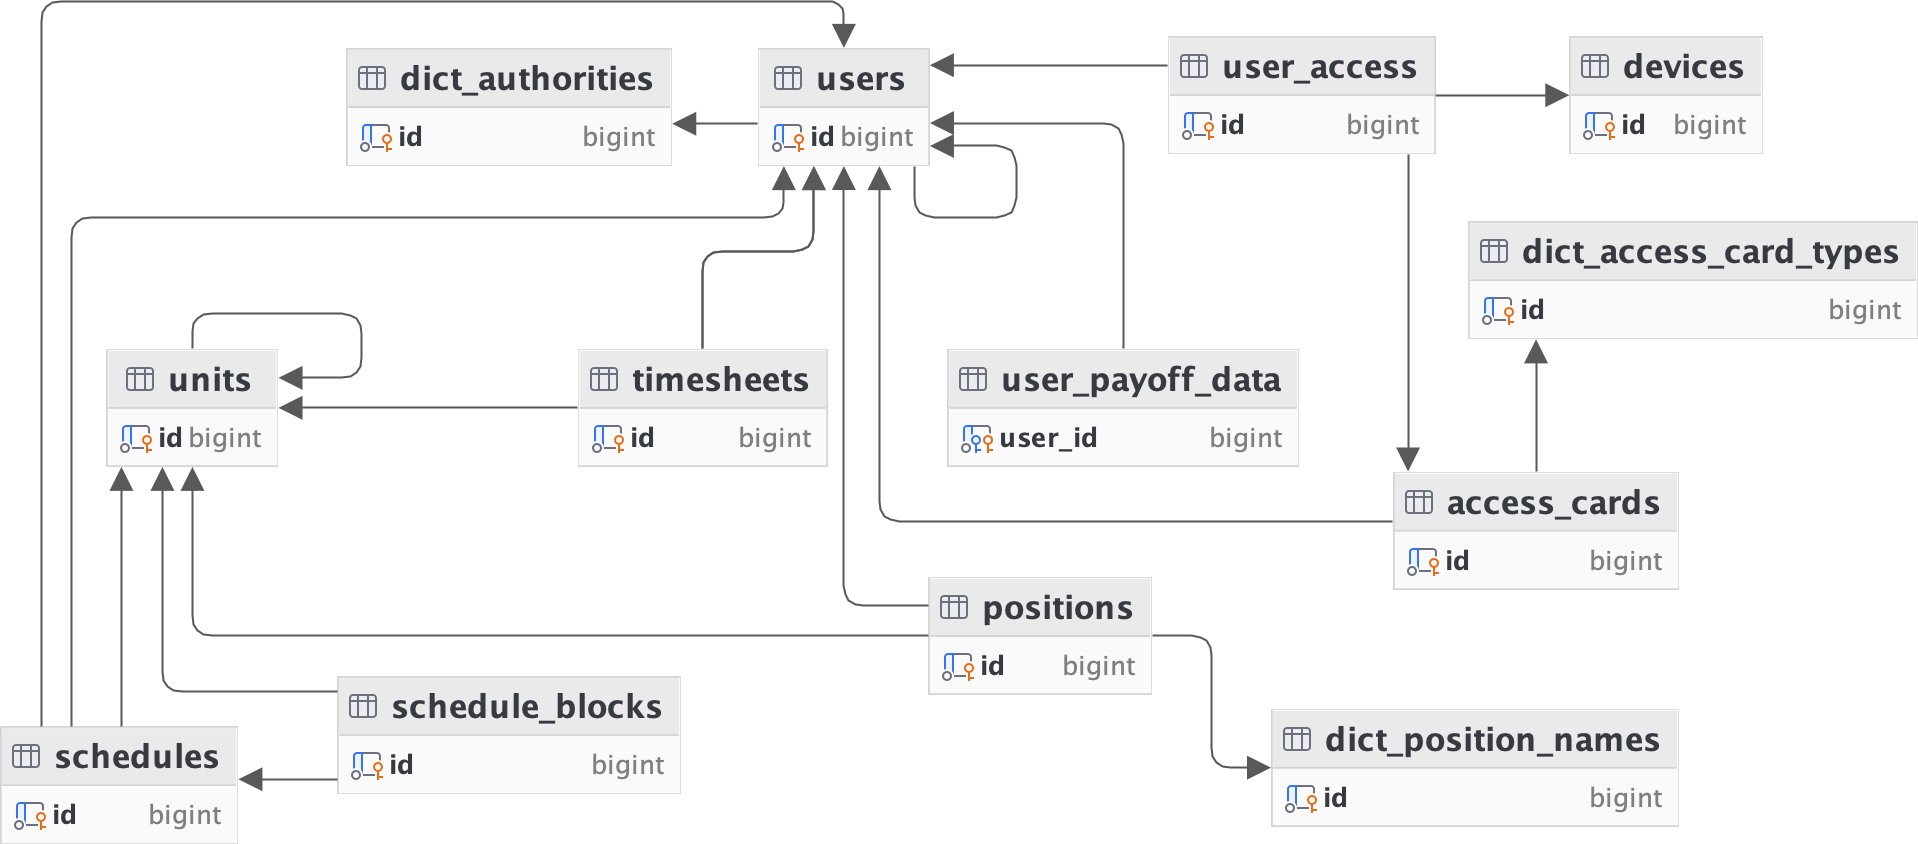
\includegraphics[width=\textwidth]{graf/dbDiagram.png}
    \caption{Uproszczony schemat bazy danych}
    \label{fig:dbDiagram}
\end{figure}

\subsection{Tabele użytkowników}

Główną tabelą przechowującą informacje o użytkownikach jest tabela \texttt{USERS}. Zawiera ona dane personalne, takie jak imię, nazwisko, adres e-mail i numer telefonu. Dodatkowo do tabeli wpisane są dane do logowania: nazwa użytkownika i hasło; oraz informacja o użytkowniku, który utworzył dany wpis. Każdy użytkownik ma przypisaną jedną z ról z tabeli \texttt{DICT\_AUTHORITIES}, która określa jego uprawnienia w systemie. Relacją jeden do jednego jest połączona tabela \texttt{USER\_PAYOFF\_DATA} zawierające dane o koncie bankowym użytkownika. W tabeli \texttt{USERS} znajduje się również pole \texttt{is\_archived}, które określa, czy użytkownik jest aktywny w systemie. Przedstawienie graficzne tabel użytkowników znajduje się na rysunku \ref{fig:usersTable}.

\begin{figure}[H]
    \centering
    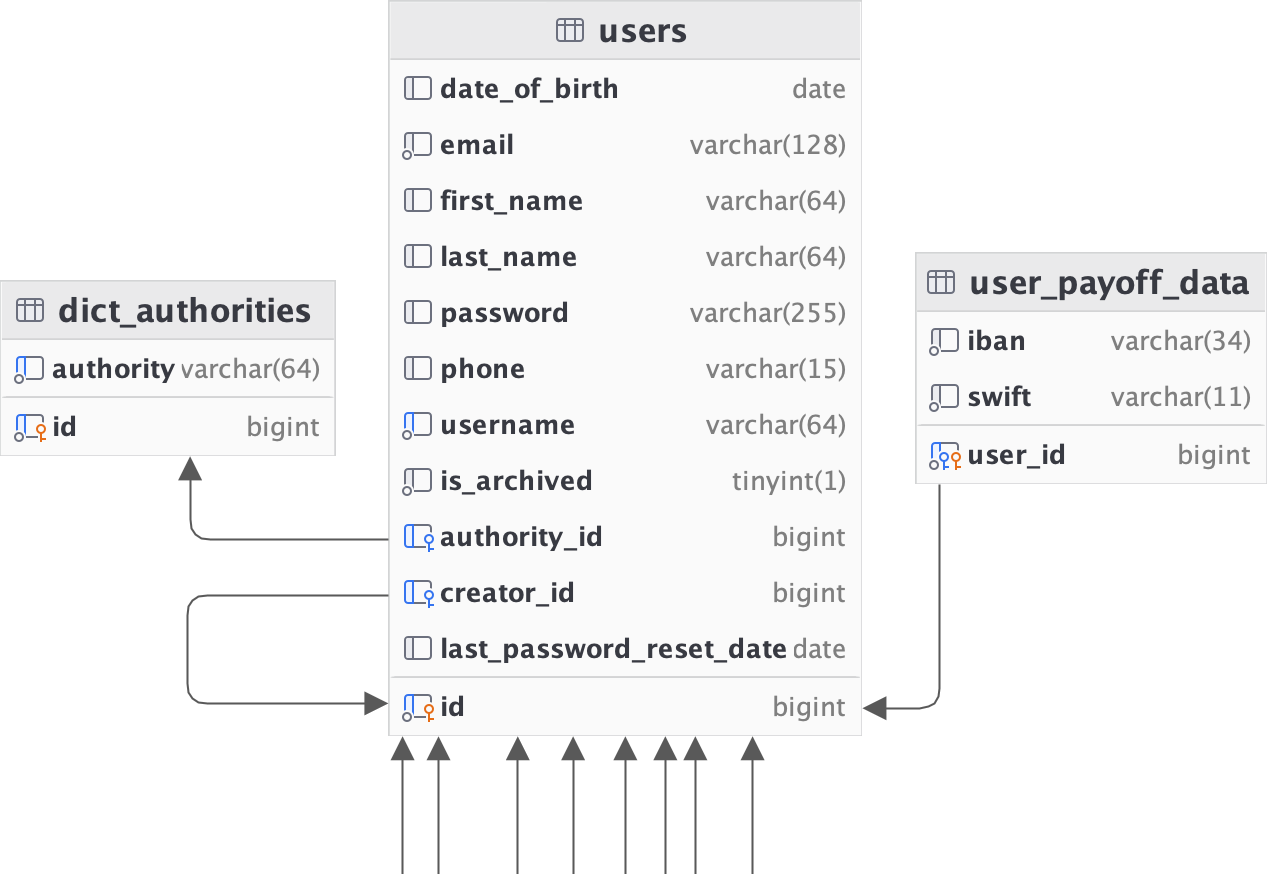
\includegraphics[width=0.7\textwidth]{graf/usersTable.png}
    \caption{Schemat tabel użytkowników}
    \label{fig:usersTable}
\end{figure}

\subsection{Tabele jednostek organizacyjnych}

Wszystkie jednostki organizacyjne są przechowywane w tabeli \texttt{UNITS} zawierającej dane o nazwie jednostki, jej opisie, jednostce nadrzędnej oraz dacie utworzenia. Pole \texttt{work\_ended} określa, czy jednostka jest aktywna. Użytkownicy są przypisani do jednostki organizacyjnej poprzez tabelę \texttt{positions} będącą tabelą łącznikową między tabelami \texttt{USERS} i \texttt{UNITS}. Znajdują się w niej dane o dacie rozpoczęcia pracy na danym stanowisku oraz dacie zakończenia pracy, a także odwołanie do tabeli słownikowej, zawierającej nazwy stanowisk. Tabela \texttt{POSITIONS} jest szczególnie ważna przy odczytywaniu harmonogramów pracy. Schemat tabel jednostek organizacyjnych został przedstawiony na rysunku \ref{fig:organizationalUnitsTable}.

\begin{figure}[H]
    \centering
    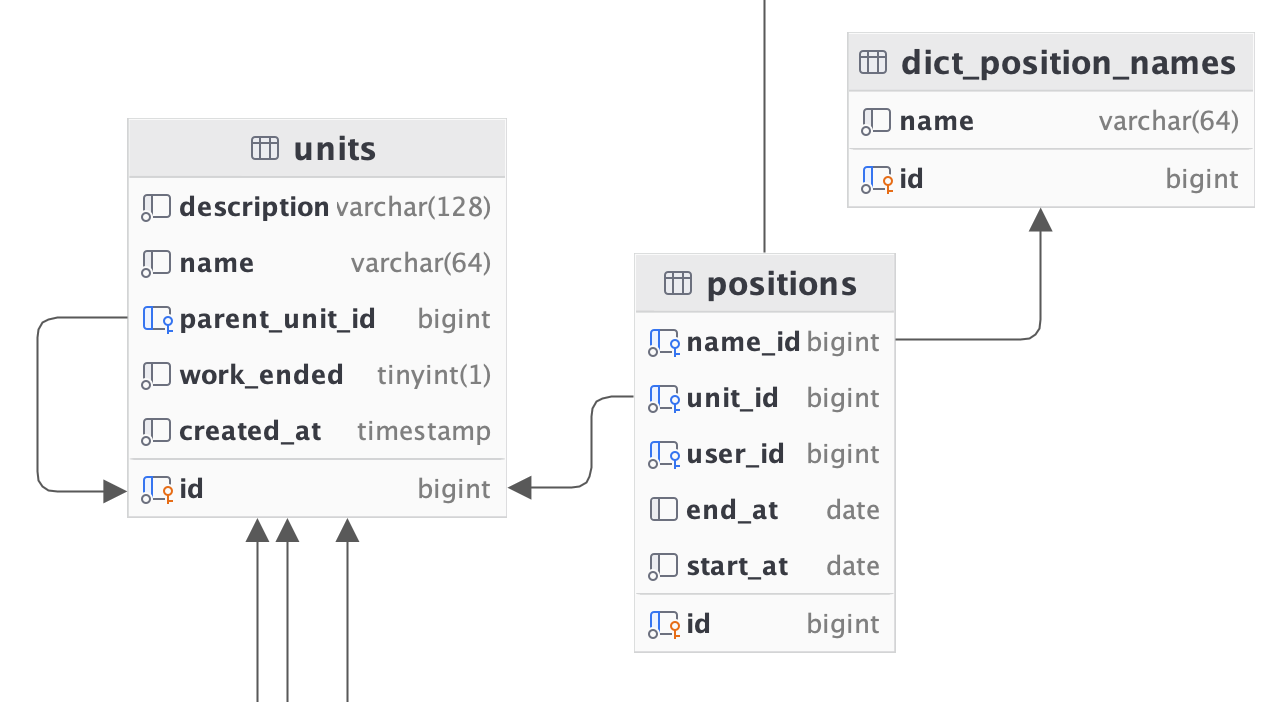
\includegraphics[width=0.8\textwidth]{graf/unitsTable.png}
    \caption{Schemat tabel jednostek organizacyjnych}
    \label{fig:organizationalUnitsTable}
\end{figure}

\subsection{Tabele harmonogramów}
\label{ss:harmonogramy}


Na każdy z harmonogramów składa się pojedynczy rekord w tabeli \texttt{SCHEDULES} oraz pewna liczba rekordów w tabeli \texttt{SCHEDULE\_BLOCKS}. Pierwsza z nich zawiera informacje o dacie rozpoczęcia i zakończenia harmonogramu, jego utworzenia oraz odwołanie do jednostki organizacyjnej lub użytkownika, którego dotyczy. Tabela \texttt{SCHEDULE\_BLOCKS} odpowiada za przechowywanie pojedynczych bloków czasowych w harmonogramie opisując jednostkę, której dotyczą, a także ich dzień i godzinę rozpoczęcia oraz zakończenia. Blok nie musi odpowiadać jednostce organizacyjnej, do której przypisany jest cały harmonogram. Tabele są powiazane relacją jeden do wielu - jeden harmonogram może zawierać wiele bloków czasowych. Przedstawienie tabel harmonogramów widoczne jest na rysunku \ref{fig:schedulesTable}.

\begin{figure}[H]
    \centering
    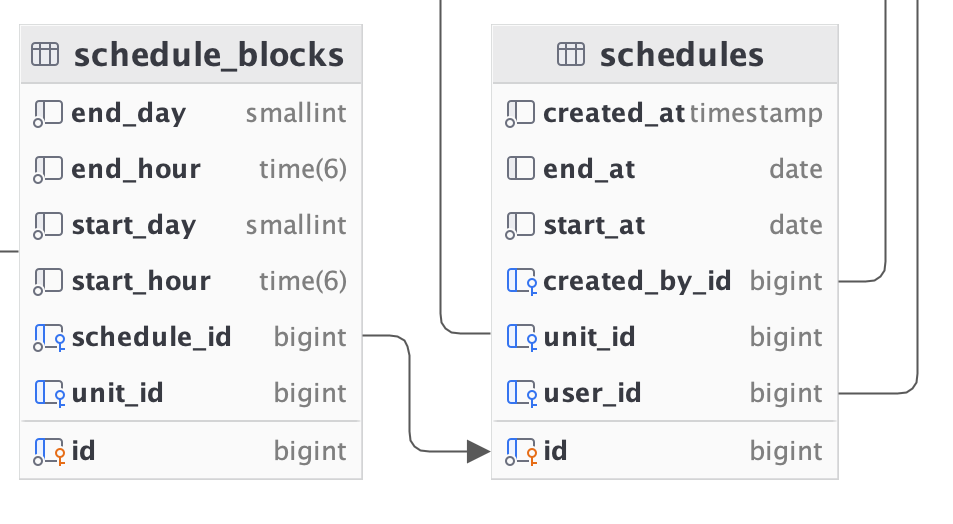
\includegraphics[width=0.7\textwidth]{graf/scheduleTable.png}
    \caption{Schemat tabel harmonogramów}
    \label{fig:schedulesTable}
\end{figure}

\subsection{Tabele kart dostępowych}

Karty dostępowe użytkowników są przechowywane w tabeli \texttt{ACCESS\_CARDS} zawierającej informacje o numerze seryjnym, jej właścicielu, opisie, typie karty oraz statusie. Dzięki ostatniej z właściwości możliwe jest przypisanie dwóm użytkownikom jednej karty w różnych okresach czasu. Każda autoryzacja użytkownika jest zapisywana w tabeli \texttt{USER\_ACCESS} wpisując do niej datę i godzinę, id użytkownika, id czytnika, id karty dostępowej oraz status autoryzacji. Umożliwia to późniejsze analizowanie historii dostępu. Wizualizacja tabel kart dostępowych znajduje się na rysunku \ref{fig:accessCardsTable}.

\begin{figure}[H]
    \centering
    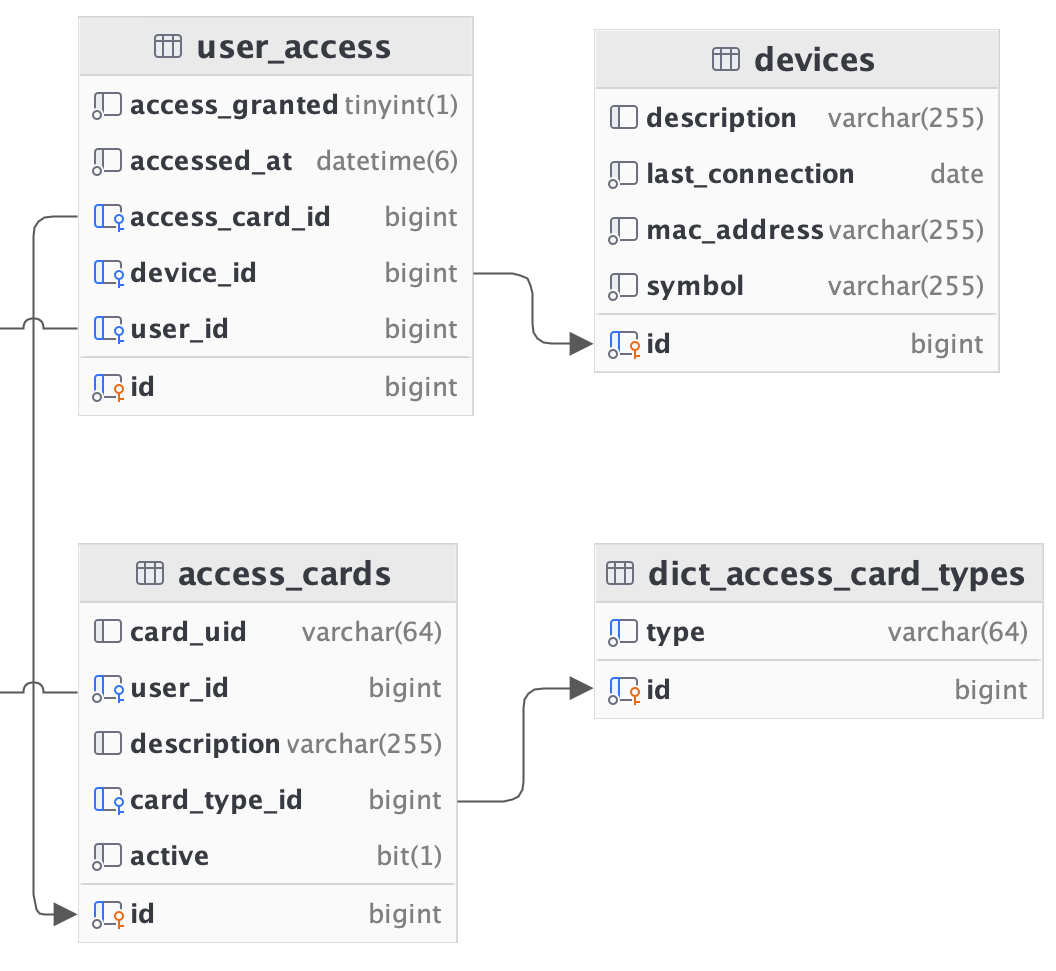
\includegraphics[width=0.7\textwidth]{graf/acTable.png}
    \caption{Schemat tabel kart dostępowych}
    \label{fig:accessCardsTable}
\end{figure}

Tabela \texttt{DEVICES} przechowuje informacje o czytnikach kart - ich opis, datę ostatniego uruchomienia, adres MAC (ang. \english{Media Access Control address}) oraz symbol, którym identyfikuje się w systemie.

\subsection{Tabele słownikowe}

W bazie danych znajdują się trzy tabele słownikowe zawierające dane, które nie zmieniają się w czasie działania systemu. Każda z nich poprzedzona jest prefiksem \texttt{DICT\_}. Są to:
\begin{itemize}
    \item \texttt{DICT\_AUTHORITIES} zawierająca role użytkowników, równoznaczne z uprawnieniami,
    \item \texttt{DICT\_ACCESS\_CARD\_TYPES} zawierająca typy kart dostępowych dla łatwiejszego rozróżnienia tagów NFC,
    \item \texttt{DICT\_POSITION\_NAMES} zawierająca nazwy stanowisk przypisanych pracownikom.
\end{itemize}

Do tabel \texttt{DICT\_ACCESS\_CARD\_TYPES} i \texttt{DICT\_POSITION\_NAMES} mogą zostać dodane nowe rekordy, lecz nie jest możliwe ich usunięcie. Takie ograniczenie zapewnia integralność danych w systemie i zapobiega błędom w działaniu aplikacji.

Dane mogą dodawać jedynie administratorzy systemu.

\section{Modele i struktury danych}

% \note{W tej części pracy należy opisać, jakie modele danych zostały zastosowane w systemie. Należy zaznaczyć, jakie są relacje między nimi.}

Dzięki użyciu w projekcie JPA (ang. \english{Java Persistence API}) oraz Hibernate, struktury danych w systemie odpowiadają strukturom tabel w bazie danych - każda z tabel bazy danych jest mapowana na odpowiadającą jej klasę w systemie. Oprócz tego zostały zaimplementowane klasy pomocnicze oraz klasy DTO (ang. \english{Data Transfer Object}),

\subsection{Klasy encji}

Zaimportowane zależności w projekcie umożliwiają tworzenie klas encji, które są mapowane na tabele w bazie danych. Każda z nich posiada adnotację \texttt{@Entity} - informującą JPA o tym, że klasa jest encją - oraz \texttt{@Table} z nazwą tabeli, z którą jest mapowana. Każde pole klasy, które odpowiada kolumnie w tabeli jest odpowiednio oznaczone. Do generowania metod \texttt{get} i \texttt{set} używane są adnotacje \texttt{@Getter} i \texttt{@Setter} z biblioteki \texttt{lombok}. W klasach znajdują się również proste, publiczne metody przetwarzające dane, dzięki którym możliwe było uproszczenie logiki biznesowej.

\subsection{Klasy pomocnicze}

Aby zapewnić poprawne działanie systemu, niezbędne było zaimplementowanie klas pomocniczych. Nie są one mapowane na tabele w bazie danych, a ich celem jest uproszczenie logiki biznesowej oraz zwiększenie czytelności kodu. Dzielą się na dwie kategorie: narzędziowe oraz danych.

Klasy należące do pierwszej z kategorii zawierają jedynie metody statyczne i nie wymagają tworzenia instancji ich obiektu. Istnieją dwie takie klasy:
\begin{itemize}
    \item \texttt{DateUtils} - zawierająca metody do zmiany dat z formatu \texttt{java.time.LocalDate} na \texttt{java.util.Date} oraz \texttt{java.sql.Date},
    \item \texttt{JwtTokenUtils} - zawierająca metody do generowania, weryfikacji i wyłuskiwania danych z tokenów JWT.
\end{itemize}

Druga kategoria klas pomocniczych to klasy danych, które istnieją w celu uproszczenia przechowywania danych w systemie. Służą najczęściej jako kontenery na dane, które następnie zostaną przetworzone na obiekty klas DTO. Najważniejszą z nich jest klasa \texttt{Calendar}, reprezentująca harmonogramy w formie kalendarza. Przechowuje ona dane dla każdego dnia tygodnia w ustalonym przedziale czasowym i dodatkowo posiada metody do sortowania, nadpisywania dni oraz uzupełniania pustych miejsc w kalendarzu.

\subsection{Klasy DTO}

W pakiecie \texttt{apimodels}, odrębnym od głównego pakietu serwera znajdują się definicje klas DTO. Służą one do ustalania struktury obiektów przesyłanych między serwerem a klientem, zapewniając poprawne działanie systemu. Każda z nich jest zaimplementowana jako klasa Java, która posiadaja jedynie publiczne pola dostępowe. Nie jest na nich wykonywana żadna logika biznesowa, a dane są wpisywane bezpośrednio przed przesłaniem ich do odbiorcy.

Pakiet apimodels zawiera subpakiety odpowiadające kontrolerom, które wymagają przesłania pełnego obiektu. Są to:
\begin{itemize}
    \item \texttt{access\_card} - modele kart dostępowych,
    \item \texttt{auth} - modele autoryzacji i autentykacji,
    \item \texttt{schedule} - modele harmonogramów,
    \item \texttt{timesheet} - modele timesheetów,
    \item \texttt{unit} - modele jednostek organizacyjnych,
    \item \texttt{user} - modele użytkowników.
\end{itemize}

\section{Algorytmy}

\subsection{Rejestracja i pierwsze logowanie użytkownika}

Rejestracja użytkownika może zostać dokonana jedynie przez administratora systemu. W tym celu powinien on wypełnić formularz rejestracyjny wprowadzając nazwę użytkownika oraz jego adres email. Po zatwierdzeniu formularza, w widoku wszystkich użytkowników pojawi się nowy rekord z danymi właśnie utworzonego użytkownika. Następnie administrator powinien przekazać nowo zarejestrowanemu użytkownikowi jego nazwę, którą musi wpisać na ekranie logowania - nie jest wymagane przy tym wpisywanie hasła. Po zatwierdzeniu formularza, i wysłaniu danych do serwera, zostanie sprawdzone czy użytkownik o podanej nazwie istnieje w bazie danych i czy ma przypisane hasło. Jeżeli nie, zwróci kod 206 - \texttt{Partial Content}, a aplikacja udostępni użytkownikowi możliwość ustawienia hasła. Po jego wpisaniu, potwierdzeniu i zatwierdzeniu formularza, użytkownik zostanie zalogowany do systemu. Diagram sekwencji pierwszego logowania użytkownika został przedstawiony na rysunku \ref{fig:login}, a szczegóły tego procesu zostały opisane w rozdziale \ref{ss:logowanie}

\subsection{Logowanie}
\label{ss:logowanie}

Logowanie do systemu odbywa się poprzez przesłanie żądania HTTP z danymi logowania do serwera aplikacyjnego. Po jego otrzymaniu serwer zwraca się do bazy danych w celu znalezienia użytkownika o podanej nazwie. Jeżeli użytkownik nie istnieje, serwer zwraca kod błędu 401. W przeciwnym wypadku sprawdza, czy zahashowane hasło użytkownika jest zgodne z zapisanym w bazie. Jeżeli hasła się zgadzają, serwer generuje dwa tokeny JWT (ang. \english{JSON Web Token}) i zwraca je w odpowiedzi. Aplikacja kliencka zapisuje otrzymane tokeny w pamięci lokalnej przeglądarki i przechodzi do widoku panelu głównego. Diagram czynności logowania został przedstawiony na rysunku \ref{fig:login}.

\begin{figure}[H]
    \centering
    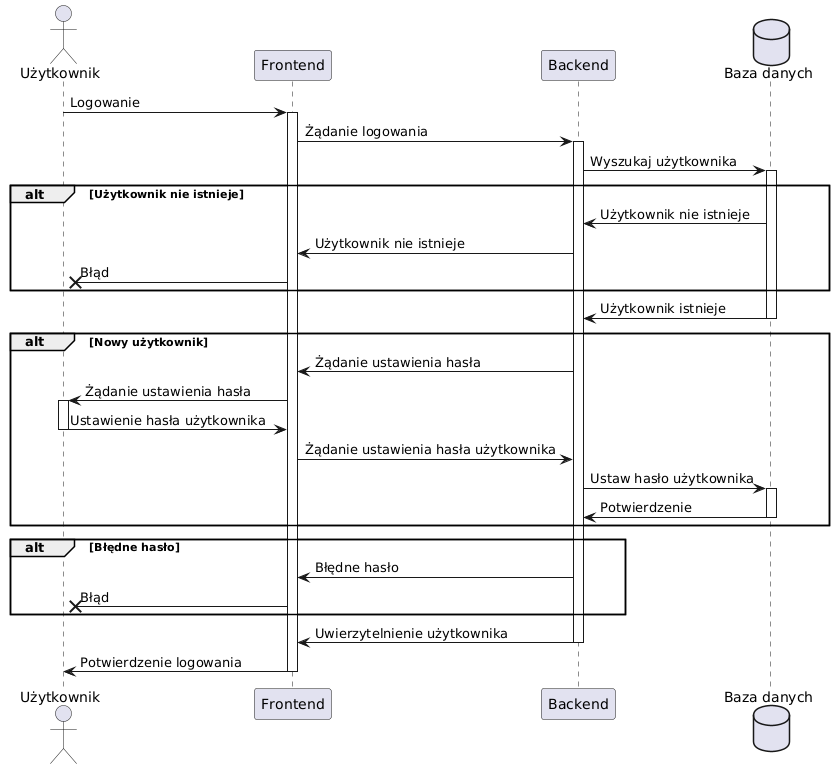
\includegraphics[width=0.9\textwidth]{graf/loginSequence.png}
    \caption{Diagram czynności logowania}
    \label{fig:login}
\end{figure}
% //www.plantuml.com/plantuml/png/VP8nRiCm34LtdKB8dWju288CdOgYIz2PigX6iIC5jbJN7WFq43rBEzRtAeceK6pKcJpyh__9Hs_R04s8frf06NmZz-Dt7ohVELj9QAMBuaowBUqPN90FZNS1dMR9u4JQGLabHQ7G4411YtArWm6a1jUNXnMBMWaXN9Jh3IN8GZxwLz-1iyW3s3S8oCa6rnl5ylZryw5PbdKoGZPIaK9EqegiBtqxn0gECkOTifcBeGwJ1JdMje4-HnfPSHANBdfIcxdhCUnv9t9aseqN6byG5uhdZMOFSpdEvtpoNN-xYL24n4oHH3fUPv6Oo0EqumK4StFnhYaZuUkwoAd5_i-4oJI5gF7cJJfEiLmnUysJQqMRi-tgy8j7Ig0A-Um3PJPweDmv80RAa9ZlftQOGZEZkM3mdvja-vwRXZvWxQuGbhPNwRuSDHin_w2t3moABLN5K_qB

\subsection{Uwierzytelnianie użytkownika}

Klient po zalogowaniu się do systemu otrzymuje od serwera dwa tokeny JWT, które są przechowywane w pamięci lokalnej przeglądarki. Aby mógł korzystać z zasobów serwera, musi dołączać pierwszy z nich - token dostępowy - do nagłówka każdego żądania HTTP pod kluczem \texttt{Authorization} poprzedzając go słowem \texttt{Bearer}. Token ten jest ważny przez określony czas, po którym traci ważność - serwer symbolizuje to kodem błędu 401. Jeżeli zaistnieje taka sytuacja, klient musi wysłać żądanie odświeżenia tokena do serwera dołączając drugi token - odświeżający - który ma dłuższy czas przedawnienia. Serwer następnie sprawdza, czy token odświeżający jest poprawny i zwraca nowe tokeny. W przeciwnym wypadku klient musi ponownie zalogować się do systemu. Diagram sekwencji procesu uwierzytelniania użytkownika został przedstawiony na rysunku \ref{fig:authSequence}.

\begin{figure} [H]
    \centering
    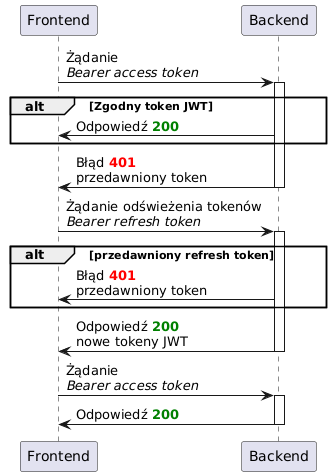
\includegraphics[width=0.4\textwidth]{graf/jwtSeq.png}
    \caption{Diagram sekwencji procesu uwierzytelniania użytkownika}
    \label{fig:authSequence}
\end{figure}
% //www.plantuml.com/plantuml/png/fPAnIiH048RxVOhX-a0KAudBaSB2naOG9CraPt8knjcmMGrdAVWKFeQTscdUopLHk1K5zQeKy__pV_zabtr07wukMzN5hpMsGmbmw9q45WBieU5aLAAv-9ZKh5J3cQuPzc5yUhqZ5CjGIM5roUZP0nh3VG_1HOz24-mr1dutOXlWREL8rlCGZavFL5oKwHWOrnrJvmRBD3v2qKGOCAvr_c2nyiooq4MjT_DSiL0qPNgobEDjH4ZbdcaIx-KxbNJ-XWa7iUupLH5lG7rNnj5u7pd6PnQBi-dbOTYiwBdnt9__q379JANRW2VDVtUiIiGDFDlNqxcJyl_-at-Z-1Agr9A5ulDx0m00

\subsection{Harmonogramowanie}

Harmonogramowanie jest częścią systemu, która pochłania najwięcej zasobów serwera - dane za każdym razem są przetwarzane na nowo. Odejście od praktyki wstępnego generowania harmonogramów i zapisywania ich w bazie danych umożliwiło zredukowanie ilości danych przechowywanych w bazie oraz konieczności ich aktualizacji w przypadku zmian w grafiku pracy.

\subsubsection{Zapis harmonogramu}

Harmonogramowanie pracy użytkowników odbywa się poprzez wysłanie żądania HTTP z danymi harmonogramu do serwera aplikacyjnego. Następnie tworzona jest struktura danych odpowiadająca tabelom opisanym w rozdziale \ref{ss:harmonogramy} i zapisywana w bazie danych. Po zakończeniu procesu, serwer zwraca kod 200 - \texttt{OK}, a aplikacja kliencka przechodzi do widoku harmonogramu.

\subsubsection{Odczyt harmonogramu}

Odczyt harmonogramu odbywa się poprzez wysłanie żądania \texttt{GET} na adres odpowiednio:
\begin{itemize}
    \item \texttt{/schedule/getUnit/\{id\}/\{startDate\}/\{endDate\}} - dla harmonogramu jednostki organizacyjnej,
    \item \texttt{/schedule/getUser/\{id\}/\{startDate\}/\{endDate\}} - dla harmonogramu użytkownika,
\end{itemize}
Uzupełniając odpowiednio parametry w nawiasach klamrowych. Oba żądania działają w podobny sposób - pierwszy z nich uwzględnia wyłącznie harmonogramy jednostki, natomiast drugi łączy harmonogramy wszystkich jednostek przypisanych do użytkownika, a następnie nadpisuje je harmonogramami użytkownika. W odpowiedzi serwer zwraca dane w formacie \texttt{JSON}, które są przetwarzane przez aplikację kliencką i wyświetlane w odpowiednim widoku.

Odczytanie harmonogramu użytkownika jest dużo bardziej złożone niż jednostki organizacyjnej. Wymaga ono odczytu wszystkich jednostek, do których należał użytkownik w danym okresie czasu, następnie dla każdej z nich odczytania harmonogramu i połączenia ich w jeden widok przechowywany w klasie pomocniczej \texttt{Calendar}. Jeżeli użytkownik posiada również własny harmonogram, serwer generuje jego widok i nadpisuje dane przechowywane w klasie. Diagram sekwencji tego procesu został przedstawiony na rysunku \ref{fig:scheduleSequence}.

\begin{figure}[H]
    \centering
    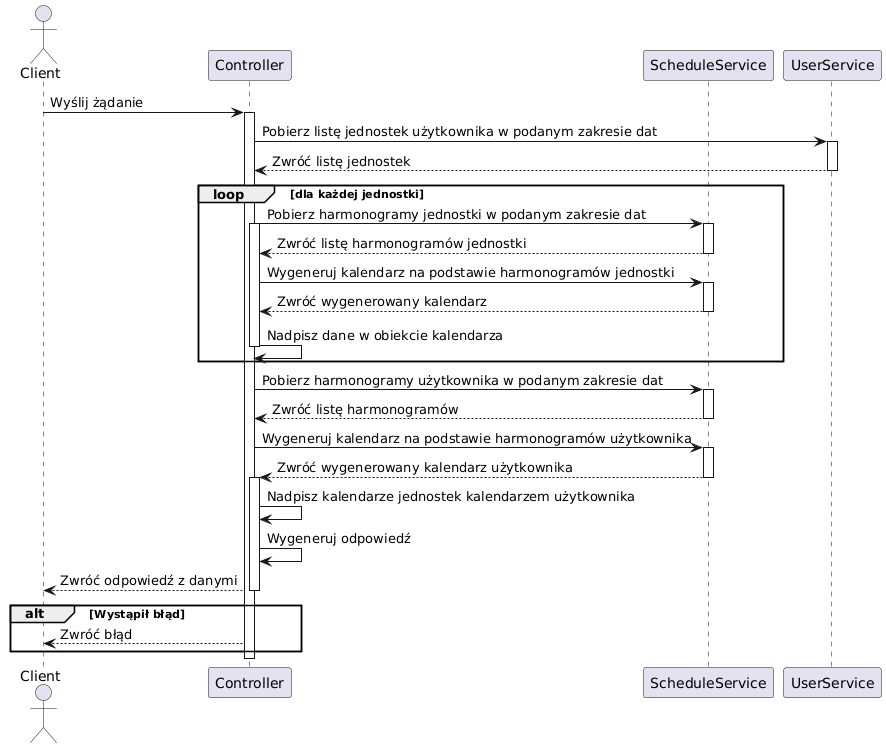
\includegraphics[width=\textwidth]{graf/schSeq.png}
    \caption{Diagram sekwencji odczytu harmonogramu użytkownika}
    \label{fig:scheduleSequence}
\end{figure}
% //www.plantuml.com/plantuml/png/dPJFQXin4CRlynH3xdw1749WxwKWJA6toMf8vDLAYrREOXy3fizG-XYv5T_YVQ-EDhXQkTWizMtdppU_-IJviOyKuhQr05H77x2oXbr4wd7TSm3e96rgqv44xohlOl3MShXB5LMPLVKBwwrbnU7Lr3oLA5NM9D5vVgq0KWnN3rZTuxVT-CkQ3Ox7qq6JCvoep2j5bc5GIPLqtEDN_sGuxD6QFfv-ueQrytta1hVZSHSRFpZJ40xOUH7PjRYd9d1l63N5h2YprmfNdvE_3-7Z_VJZ7qdGF6y0wts7sX8sD1urRywLZG6KtuIePeWl55hl_7EWTfThhx4bYRnn-QdKzAsk8SycVRmF5roQIvrCAfu_i-EmtSXAbfqceNQK-Ff8W-4RmelmXazzFyYwUSGjAcd-Ghep_Hx58yO1avbDRJZtqwL01P80k7a02-z7HbfeDfIB_A-r1Lx1iTJLKg6acZ-bQlLGuL-NSp_Ftb8EjgKid0yfh-TrvsKVFVwUif9EZphJvZpkSVBS01I71sIZ28gvXywCR_WqlfqE-dmdBWNFQG6ya7cKKFex-mC0

\subsection{Przypisanie  karty dostępowej}
\label{sec:addNfc}

Przypisanie karty dostępowej odbywa się przy wykorzystaniu aplikacji mobilnej. Po zalogowaniu się do systemu administrator powinien wybrać zakładkę \texttt{CARDS}, a następnie rozpocząć skanowanie tagu NFC. Po pozytywnym odczytaniu danych aplikacja wyśle do serwera żądanie o informacje na temat karty, a w kolejnym kroku wyświetli informacje jej właścicielu. Jeżeli karta jest już przypisana do użytkownika, aplikacja umożliwi jej usunięcie, a w przeciwnym wypadku udostępni listę rozwijaną z jego wyborem. Po zatwierdzeniu, aplikacja wyśle do serwera żądanie przypisania karty do użytkownika i otrzyma odpowiedź. Diagram sekwencji przypisania karty dostępowej został przedstawiony na rysunku \ref{fig:assignCard}.

\begin{figure}[H]
    \centering
    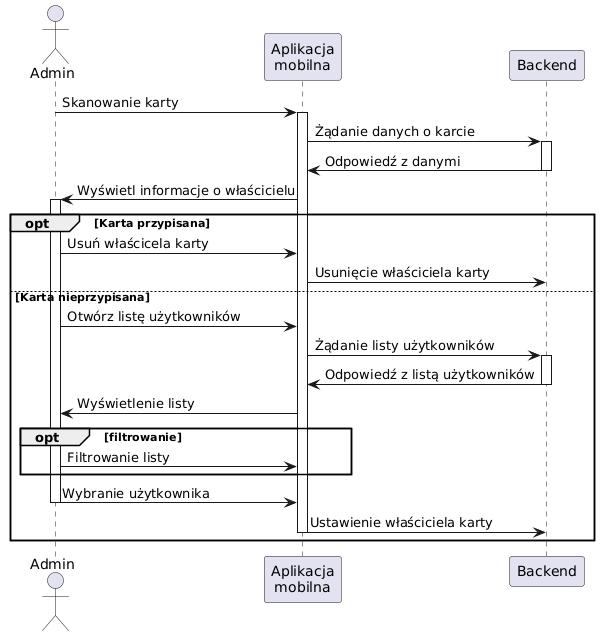
\includegraphics[width=0.7\textwidth]{graf/cardSeq.png}
    \caption{Diagram sekwencji odczytu i przypisania karty dostępowej}
    \label{fig:assignCard}
\end{figure}
% //www.plantuml.com/plantuml/png/TP8nKiCm44LxdM8dVIv0aKaeQ2XIC0mDpThQ38jbIMFBU9oI8OV8v1ZfW2xnlTW8W-r0YgY8tlx_zylpCc0HgjmeJ8ChOA5pje0be5PURZXbZpR0PE4DPvW-uwFDNSB6uYHYte-uQqmpilfqbP1IgASpGU0AxZAqhaRB19dmpScFNp1Gb93VT9QGSEt7SQCZ9cUJFe4xyIbJFo32WavdyAsyrDxLJBfzXtKSobbf6j9H7RMm3qsx4pOOOBjoHIuBaJZKxIkskvJ5nbI3P5ev7-1MyYBuOjruBj6Y0kZtkY-hzgqN88FTVW3zKW9PFcv5Vc3LesHAwbnayGj6or0VziKQ39VXk8Mg_Mn2vchBsM5V2_bFXP5jpj5nZr5-t6BdiJaR_5jgV8DHhVJh6fjRiGb5V7NXTVzaD_t_7KrM3mbHJ8fuFSY0mmIeVn9q3GUK1FP2myD1xwERciif7_uN

\subsection{Uruchomienie czytnika kart}

Uruchomienie czytnika kart odbywa się poprzez podłączenie go do zasilania. Następnie czytnik stara się połączyć z siecią bezprzewodową, która jest zapisana w jego pamięci. Po pozytywnym połączeniu, czytnik wysyła do serwera aplikacyjnego żądanie o informacje na swój temat dołączając do niego adres MAC. Serwer zwraca informacje o czytniku, a ten przechodzi do trybu oczekiwania na odczytanie karty. Jeżeli któryś z kroków nie powiedzie się, czytnik przechodzi w stan błędu i udostępnia sieć Wi-Fi o nazwie \texttt{WMS-AP} z hasłem \texttt{123456789} w celu ręcznego skonfigurowania połączenia. Po połączeniu się innym urządzeniem z siecią czytnika, należy wpisać w przeglądarce adres \texttt{192.168.4.1} i wprowadzić dane dostępowe do sieci ogólnej. Widok strony konfiguracyjnej czytnika został przedstawiony na rysunku \ref{fig:readerConfig}. Po zatwierdzeniu formularza czytnik zapisuje dane, restartuje się i ponawia opisany wcześniej proces.

\section{Połączenie modułów czytnika kart}

Czytnik kart składa się z dwóch modułów oraz kilku elementów pasywnych. Pierwszy z modułów to mikrokontroler \texttt{Raspberry Pi Pico W} odpowiedzialny za przetwarzanie danych i komunikację z serwerem aplikacyjnym. Drugi moduł - oznaczony symbolem \texttt{RFID-RC522} - odpowiada za odczytanie tagów NFC i przekazanie ich do mikrokontrolera. Oba układy są połączone ze sobą za pomocą interfejsu SPI (ang. \english{Serial Peripheral Interface}). Schemat połączeń czytnika kart został przedstawiony na rysunku \ref{fig:readerConnection}.

Do elementów pasywnych układu należą:
\begin{itemize}
    \item Rezystory ograniczające prąd,
    \item Dioda LED RGB ze wspólną katodą, sygnalizująca stan czytnika.
\end{itemize}

Zgodnie z opisem diody do każdej anody podłączony powinien być rezystor ograniczający prąd. Zgodnie z zaleceniami producenta ich rezystancja powinny wynosić:
\begin{equation}
    \begin{cases}
        R_R=100\Omega \\
        R_G=82\Omega  \\
        R_B=47\Omega
    \end{cases}
\end{equation}
z dokładnością do $5\%$. Niemożność uzyskania rezystora dla kanału zielonego spowodowała, że połączono równolegle dostępne rezystory o wartościach $100\Omega$, $1.2k\Omega$ i $1.2k\Omega$. Dzięki temu uzyskano rezystancję równą:
\begin{equation}
    R_G = \frac{1}{\frac{1}{100}+\frac{1}{1200}+\frac{1}{1200}} \approx 85.71\Omega
\end{equation}
która odbiega od wartości zalecanej o mniej niż $5\%$.
\begin{figure}[H]
    \centering
    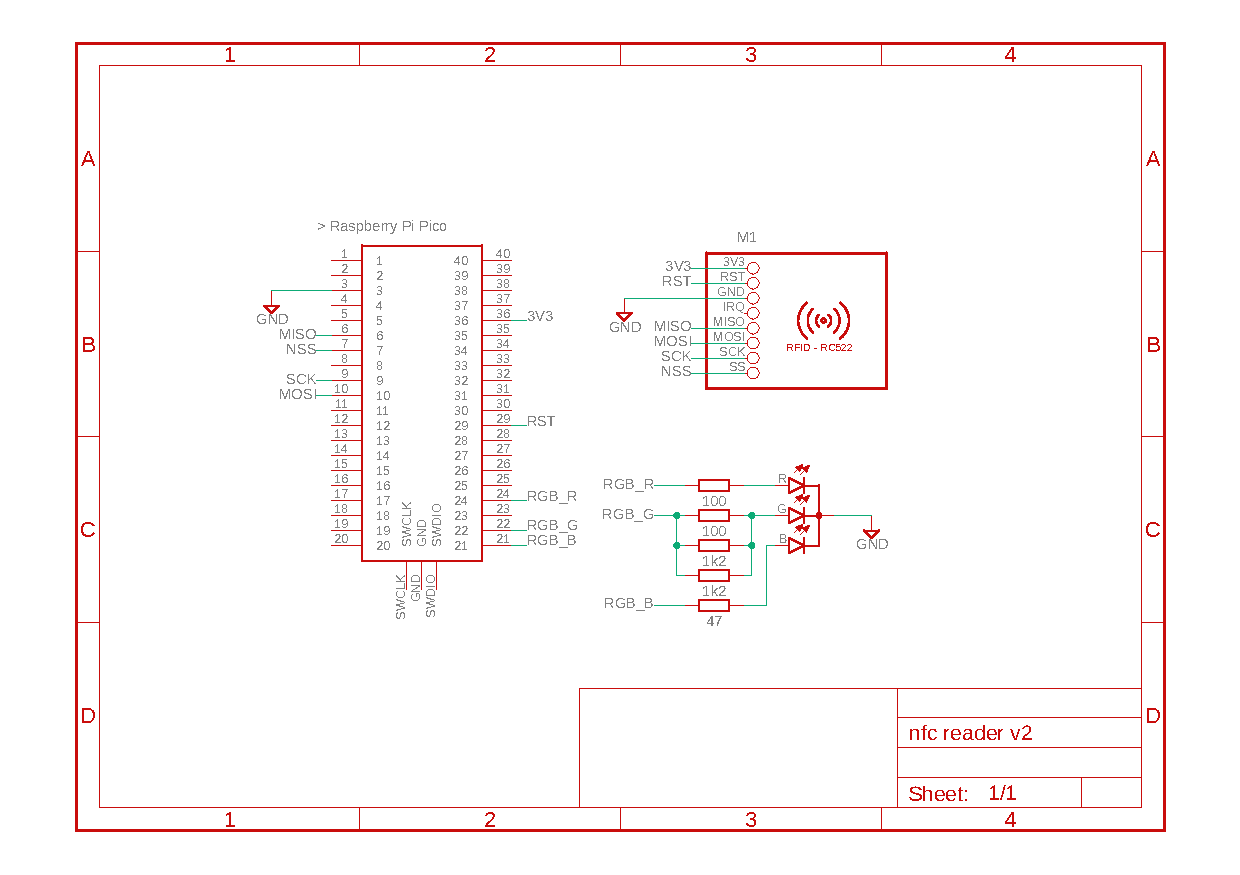
\includegraphics[width=\textwidth]{graf/nfcReader.pdf}
    \caption{Schemat połączeń czytnika kart NFC}
    \label{fig:readerConnection}
\end{figure}